\section{Building Generation}

\begin{figure}[H]
    \centering
  
    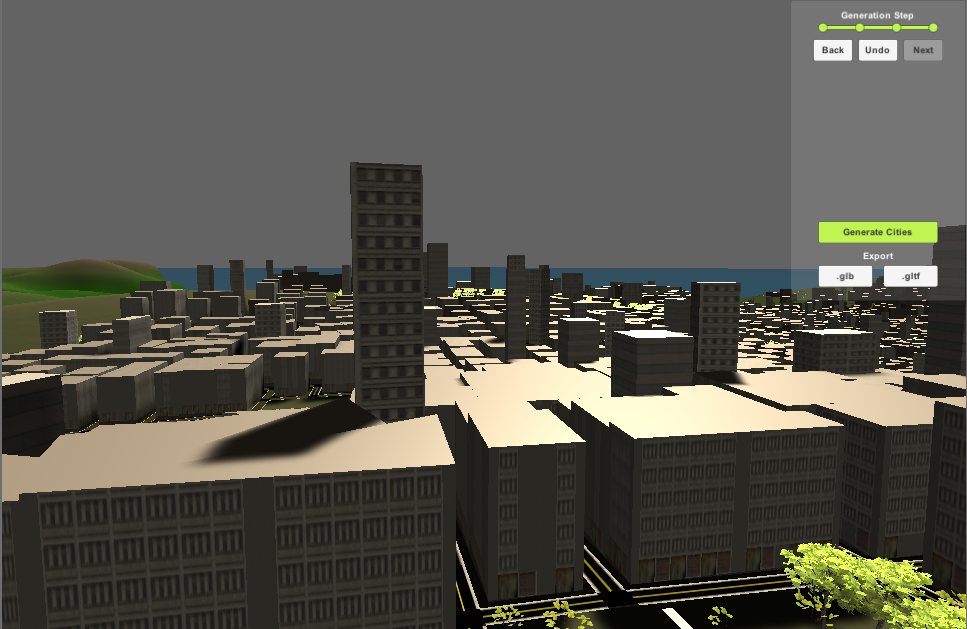
\includegraphics[width=0.7\textwidth]{figure/skyline.PNG}
    \caption{Example of a low poly triangle mesh representing a dolphin \cite{low_poly_dolphin}.}
  
    \label{fig:skyline-result}
  \end{figure}
  

  \begin{figure}[H]
    \centering
  
    \begin{subfigure}[b]{0.45\textwidth}
      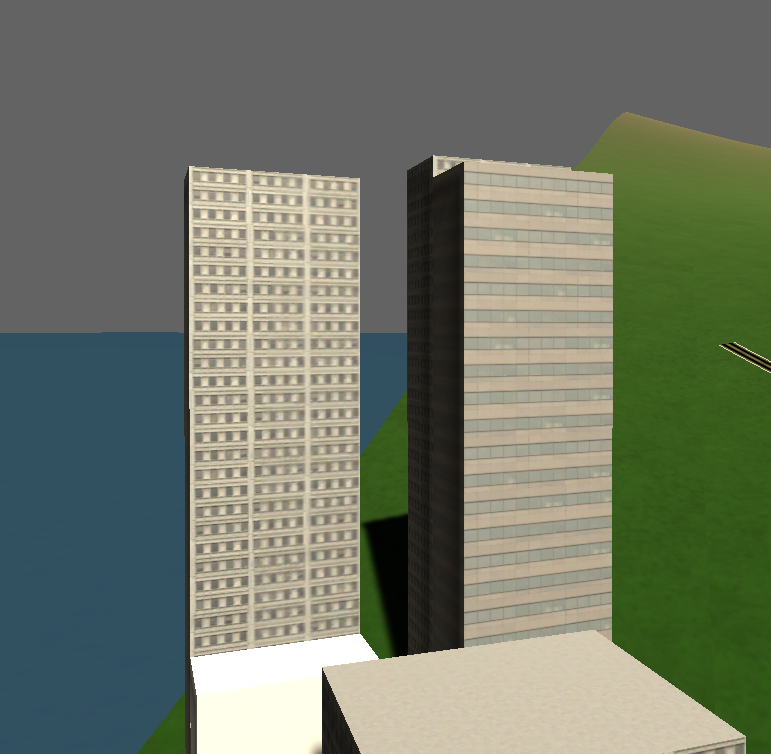
\includegraphics[width=\textwidth]{figure/skyscraper-close-up.PNG}
      \caption{\textit{EveryOtherFloor}.}
    \end{subfigure}
    \quad
    \begin{subfigure}[b]{0.45\textwidth}
      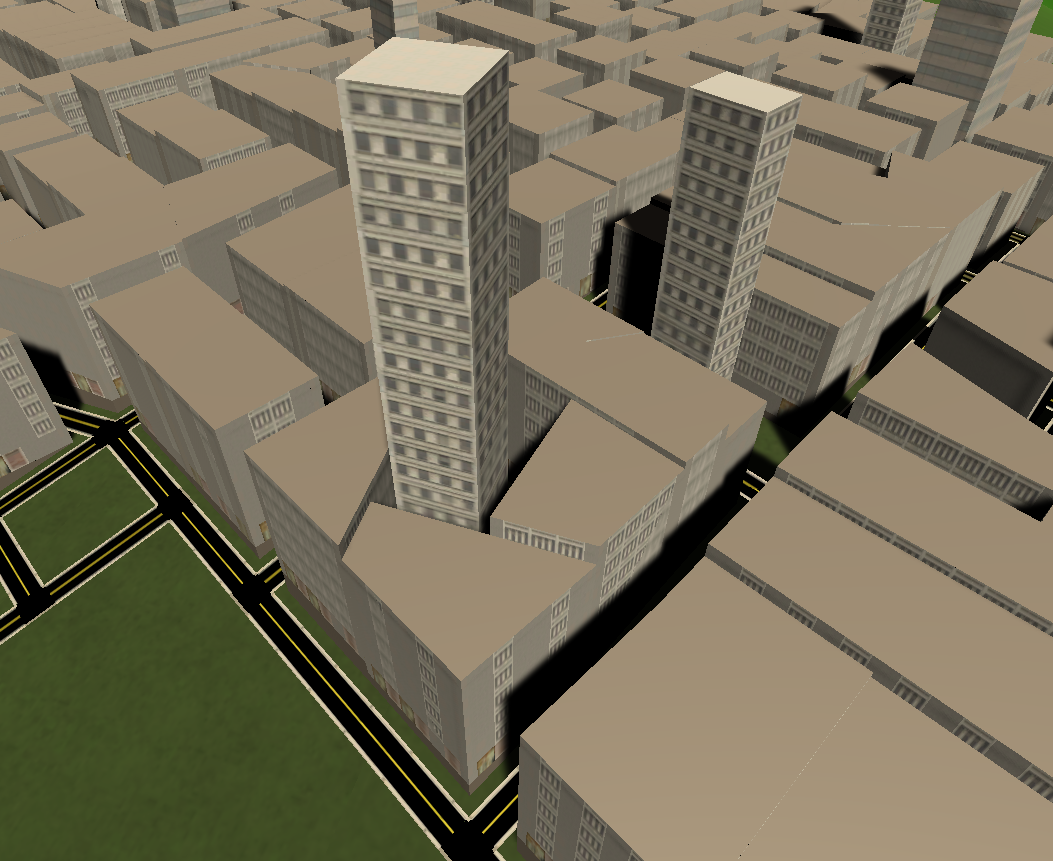
\includegraphics[width=\textwidth]{figure/wack.PNG}
      \caption{\textit{MirrorFloor}.}
    \end{subfigure}
    
    \caption{The three different wall segment generators. Notice that each building has a \textit{FirstFloor} wall segment generator on the first floor.}
    \label{fig:skyscraper-result}
  \end{figure}
  

\begin{figure}[H]
    \centering
  
    \begin{subfigure}[b]{0.25\textwidth}
      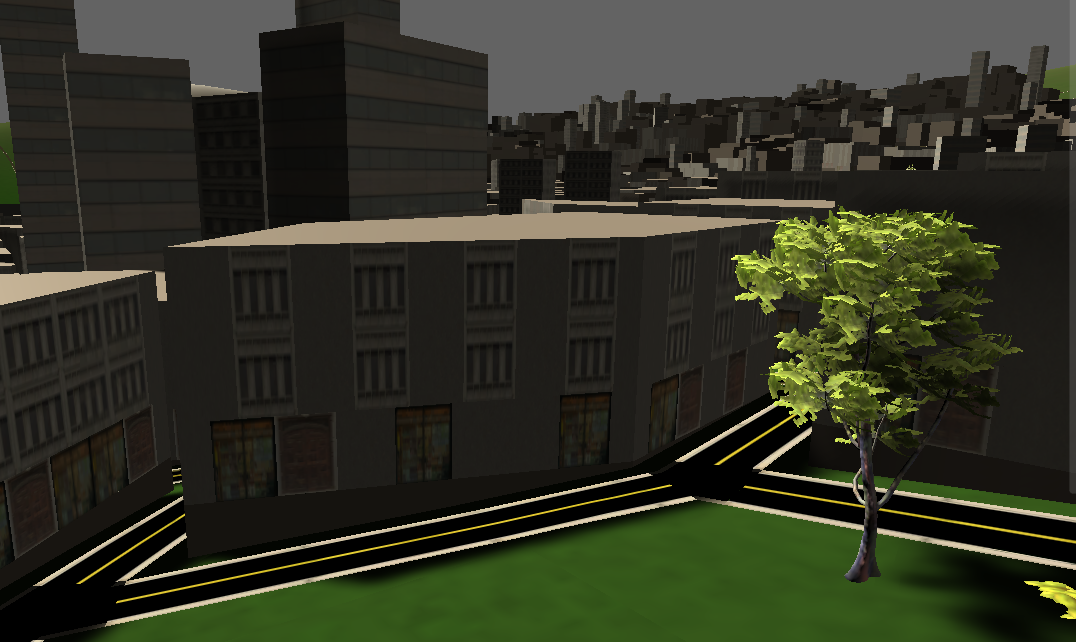
\includegraphics[width=\textwidth]{figure/building-every-other.PNG}
      \caption{\textit{EveryOtherFloor}.}
    \end{subfigure}
    \quad
    \begin{subfigure}[b]{0.25\textwidth}
      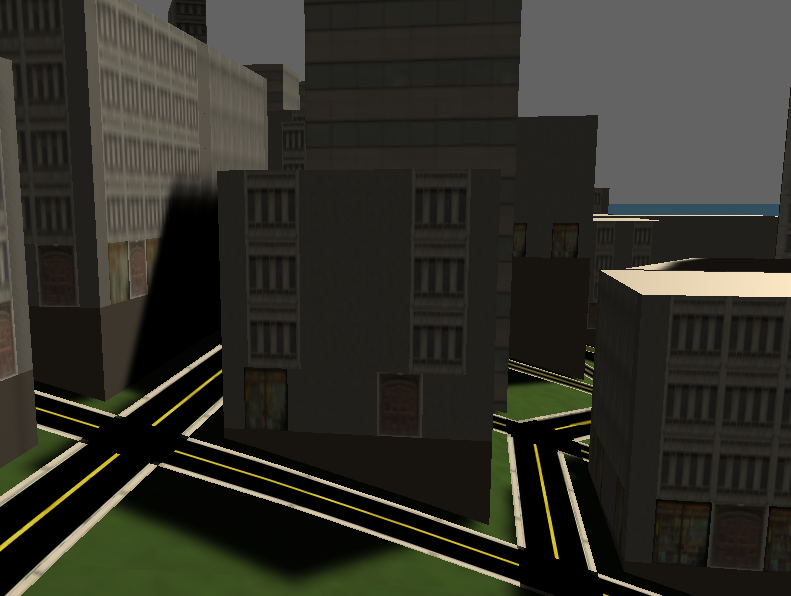
\includegraphics[width=\textwidth]{figure/building-normal.PNG}
      \caption{\textit{MirrorFloor}.}
    \end{subfigure}
    \quad
    \begin{subfigure}[b]{0.25\textwidth}
        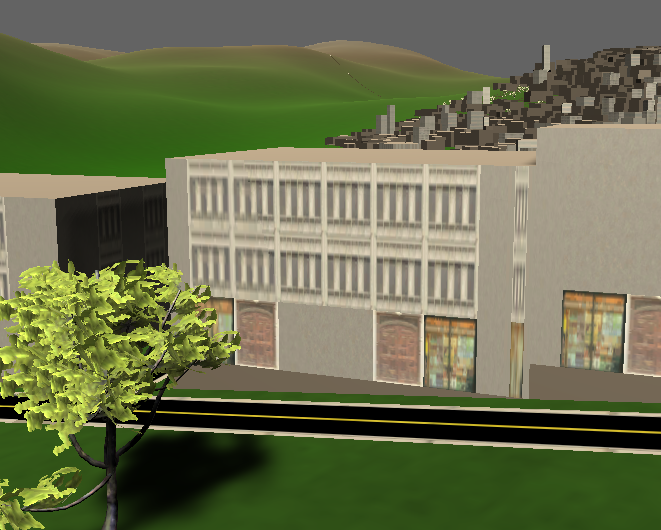
\includegraphics[width=\textwidth]{figure/building-only-window.PNG}
        \caption{\textit{OnlyWindowFloor}.}
    \end{subfigure}
    
    \caption{The three different wall segment generators. Notice that each building has a \textit{FirstFloor} wall segment generator on the first floor.}
    \label{fig:wall-segment-generator}
  \end{figure}
  